
%(BEGIN_QUESTION)
% Copyright 2006, Tony R. Kuphaldt, released under the Creative Commons Attribution License (v 1.0)
% This means you may do almost anything with this work of mine, so long as you give me proper credit

The following diagram is that of a pneumatic {\it moment-balance} differential pressure transmitter, similar to the Foxboro model 13A.  The term ``moment'' refers to the physics principle of a force acting on a lever to produce a torque.  ``Moment-balance'' is more appropriate than ``force-balance'' in this case because the device pits moment against moment, rather than force against force directly:

$$\includegraphics[width=15.5cm]{i00205x01.eps}$$

Describe this instrument's response to an increasing differential pressure (increasing pressure on the ``High'' side, and a steady pressure on the ``Low'' side; or a decreasing pressure on the ``Low'' side with a steady pressure on the ``High'' side), step by step. 

\vskip 20pt \vbox{\hrule \hbox{\strut \vrule{} {\bf Suggestions for Socratic discussion} \vrule} \hrule}

\begin{itemize}
\item{} Describe the purpose of the {\it sealing diaphragm} shown roughly mid-way along the length of the force bar.
\item{} Identify how this instrument will respond to obstructions (blockages) in the following locations:
\begin{itemize}

\item{} Nozzle
\item{} Vent (located on relay body)
\end{itemize}
\end{itemize}

\underbar{file i00205}
%(END_QUESTION)





%(BEGIN_ANSWER)

As the differential pressure increases (``high'' side pressure increases relative to ``low'' side pressure):

\begin{itemize}
\item{} Diaphragm ``capsule'' is forced to the right.
\item{} Force bar rotates counter-clockwise about the sealing diaphragm, which acts as a fulcrum for the force bar.
\item{} Flapper approaches nozzle.
\item{} Nozzle backpressure increases.
\item{} Increased nozzle backpressure presses up on relay diaphragm.
\item{} Inside relay, the ball-shaped supply valve opens and the cone-shaped vent valve closes.
\item{} Relay output pressure increases (more than the nozzle backpressure increase, due to amplification).
\item{} This output pressure is sent to the bellows, which presses to the left at the range bar's lower end.
\item{} Range bar rotates clockwise about the ``range wheel'' (movable fulcrum nut).
\item{} Top of range bar moves to the right, pulling against the force bar to move the flapper away from the nozzle.
\item{} System reaches equilibrium, where force exerted by the bellows against the range bar balances force exerted by diaphragm capsule against the force bar.
\end{itemize}

End result: output pressure equals some proportion (multiple or fraction) of differential pressure across diaphragm capsule.

%(END_ANSWER)





%(BEGIN_NOTES)


%INDEX% Measurement, pressure: Foxboro 13A pneumatic D/P cell

%(END_NOTES)


